\documentclass{article}
\usepackage{indentfirst}
\usepackage{lmodern}
\usepackage[utf8]{inputenc}
\usepackage[T1]{fontenc}
\usepackage[ngerman]{babel}
\usepackage{amssymb,amstext,amsmath}
\usepackage{graphicx}
\usepackage{dsfont}
\usepackage{amsfonts}
\usepackage{graphics}
\usepackage{float}
\usepackage{cite}
\usepackage{url}
 \usepackage{sectsty}
\usepackage{multirow}

\title{Beugung und Brechung}
\author{Alexander Heinisch, Dominik Wille}
\begin{document}
\maketitle
\vspace{13cm}
\noindent
\begin{center}
\begin{tabular}{r l}
Tutor & Katharina Klingan  \\
Durchführung & 23. April 2013 \\

E-Mail Dominik & dominik.wille@fu-berlin.de \\
E-Mail Alexander & matthias.heinisch@gmx.de \\
\end{tabular}
\end{center}

\newpage
\tableofcontents
\newpage


\section{Ziel des Versuchs}
In diesem Versuch untersuchen wir die Phänomene der Beugung und Interferenz sowie die Abbesche Theorie. Des weiteren nehmen wir den Zusammenhang zwischen einem Beugungsdiagramm und einem Bild eines Objekts unter die Lupe.\\


\section{Physikalische Grundlagen}
\subsection{Huygenssches Prinzip}
Das Huygenssche Prinzip besagt, dass bei einer Halbkreis- bzw. Halbkugelförmigen Welle jeder Punkt der Wellenfront als Ausgangspunkt einer neuen, kohärenten Elementarwelle angesehen werden kann. Dieses Prinzip ist hilfreich, wenn in Strahlengängen, quer zur Ausbreitungsrichtung von Licht o.ä., Begrenzungen oder zu große Strukturen auftreten und die Wellen gebeugt oder gebrochen werden. Zudem lassen sich damit Beugungserscheinungen und Auflösungen einer optischen Abbildung beschreiben.
Wollen wir nun die Amplitude oder die Phase in einem beliebigen Punkt wissen,  können wir das aus der Überlagerung aller Elementarwellen in diesem Punkt berechnen. \\

\subsection{Fraunhofersches Beugungsdiagramm}
Da sich bei einer Brechung sehr viele Elementarwellen überlagern, musste man sich etwas einfallen lassen, um die Beobachtung zu vereinfachen. Man betrachtet den Grenzfall einer ebenen Welle deren Quelle und Aufpunktebene sich im unendlichen befindet, was zur Folge hat, dass man die auf dem Bildschirm auftreffenden Strahlen als parallel ansehen kann. Diese Intensitätsverteilung wird als Fraunhofersches Beugungsdiagramm bezeichnet.
Experimentell lassen die eben genannten Bedingungen durch das Einsetzten von Sammellinsen realisieren, wodurch die Quelle und die Aufpunktebene eben ins endliche verschoben werden. Alternativ kann auch eine Laserlichtquelle zum Einsatz kommen, welche näherungsweise ebene Wellen abstrahlt. Die hohe Intesität des Lasers hat gleichzeitig den Effekt, dass die Aufpunktebene als hinreichend weit entfernt angenommen werden kann.\\

\subsection{Abbildung eines Objekts}
Um die Abbildung eines Objekts, welches mit parallelem Licht beleuchtet wird, zu beschreiben, verwendet man die {\sc Abbesche Theorie}.
Das ist ein zweistufiger Abbildungsvorgan, bei dem zunächst das {\sc Fraunhofersches Beugungsdiagramm} in der Brennebene der Linse entsteht,\\
welches man wiederum als Ausgangsfläche für Elementarwellen auffassen kann. Hier kommt nun wieder das {\sc Huygenssche Prinzip} zum Einsatz. Diese Elementarwellen lassen in der Bildebene das endgültige Bild des Objekts entstehen, was allerdings den Nachteil hat, dass selbst bei einfachen Objekten der Aufwand der Berechnungen umfangreich ist.\\

\subsection{Beugungsdiagramm eines Spaltes}
Da die Berechnung der Beugungsdiagramme zu schwierig sind, beschränken wir uns hier nur darauf, die Ergebnisse anzugeben und zu diskutieren. Die Intensitätsverteilung sind abhängig vom Winkel \(\alpha\) gegenüber der Ausbreitungsrichtung des Lichts. So ergibt sich für einen Einfachspalt

\vspace{0,25cm}
\begin{equation}
\label{1}
I_{Sp}(sin\ \alpha)\approx b^2 \frac{sin^2(\frac{\pi b}{\lambda}sin\ \alpha)}{(\frac{\pi b}{\lambda}sin\ \alpha)^2}
\end{equation}

\vspace{0,25cm}

für die Breite b und die Wellenlänge  \(\lambda \).
Diese Funktion wird Null für

\vspace{0,25cm}

\begin{equation}
\label{2}
sin\ \alpha = \pm n \frac{\lambda}{b}\  f"ur\ n = 1,2,3...
\end{equation}

\vspace{0,25cm}
\begin{figure}[htbp]
\centering
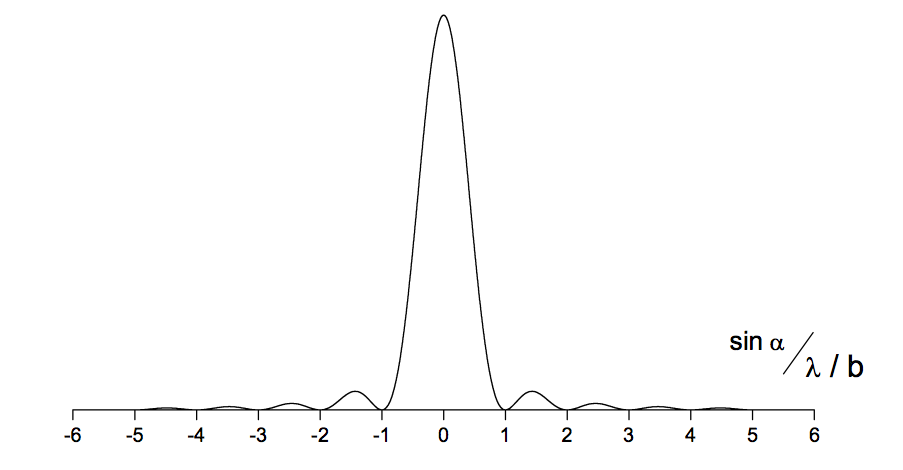
\includegraphics[scale=0.3]{BEU.png}
\begin{center}
\caption{Nullstellen der Intensität [GP 2 Skript]}
\end{center}
\end{figure}

Der Verlauf der Amplitude lässt sich aus einer gedanklichen Zerlegung des Spaltes in Teilspalte und der Betrachtung der Interferenz der benachbarten Teilbündel herleiten. Als letztes muss man nurnoch die Anzahl der Teilspalte gegen unendlich laufen lassen.

\subsection{Beugungsdiagramm des Doppelspalts}
Für den Doppelspalt setzt sich die Intensitätsverteilung aus zwei Faktoren zusammen. Der erste Faktor ist die Beugung am einfachen Spalt entsprechend \eqref{1}, während der zweite Faktor das Zusammenwirken der beiden Spalte im Abstand d ist.

\begin{equation}
\label{3}
I_{DSp} = I_{Sp}I_d = I_{Sp} cos^2(\frac{\pi d}{\lambda} sin\ \alpha)
\end{equation}

Die Extremstellen der Funktion \eqref{2} lassen sich mittels

\begin{equation}
\label{4}
sin\ \alpha = \pm n\frac{\lambda}{d}\  f"ur\ n = 1,2,3...
\end{equation}

berechnen.
Somit erhält das Beugungsdiagramm eine Folge von Maxima im Abstand $\frac{\lambda}{d}$ mit einer Höhe, welche aus der Einhüllenden bestimmt wird.

\begin{figure}[htbp]
\centering
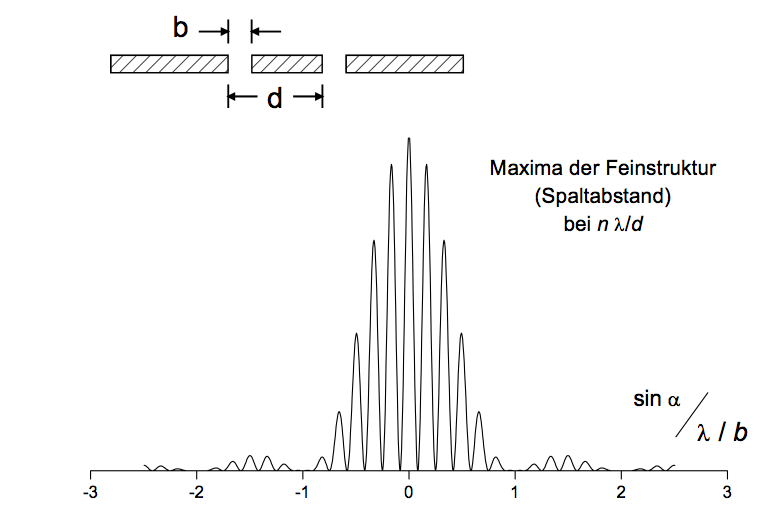
\includegraphics[scale=0.3]{BEU2.png}
\begin{center}
\caption{Nullstellen der Einhüllenden (Spaltbreite) bei n$\frac{\lambda}{b}$ [GP 2 Skript]}
\end{center}
\end{figure}

\subsection{Beugungsdiagramm des Gitters}
Es gibt keine großen Unterschiede zwischen dem Beugungsdiagramm eines Doppelspalte und eines Gitters. Die Lage der Maxima folgt Gl.\(\eqref{4}\), wobei der Spaltabstand b dabei logischer Weise durch die Gitterkonstante d ersetzt wird. Die Lage der Maxima wird hingegen durch die Größenordnung \(\frac{1}{N}\) angegeben, N entspricht hier der Anzahl der Gitterspalte. Daraus folgt, je größer N, desto schärfer sind die Beugungsmaxima.

\subsection{Beugungsdiagramm bei Reflexion an einem Gitter}
Durch die streifende Beleuchtung eines Metallmaßstabes in kleinem Winkel \(\epsilon\), benutzen wir die Skalenteilung des Maßstabes als Reflexionsgitter mit 

\begin{equation}
\label{5}
d \cdot (cos \varepsilon - cos( \varepsilon + a)) = z \lambda \ für \ z\ \varepsilon \ \mathds{Z}
\end{equation}

(d ist der Teilungsabstand des Gitters)

\begin{figure}[htbp]
\centering
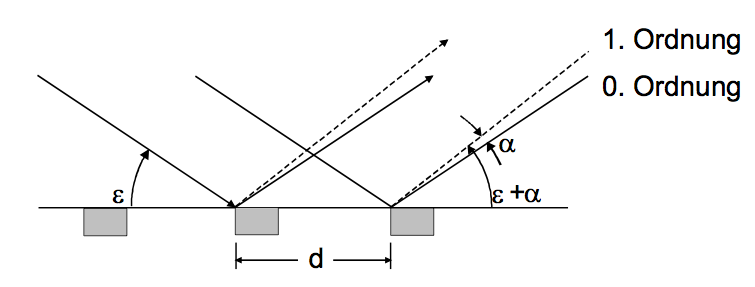
\includegraphics[scale=0.3]{BEU3.png}
\begin{center}
\caption{Reflextion am Gitter [GP 2 Skript]}
\end{center}
\end{figure}

\subsection{Grundlagen und Aufbau eines He-Ne-Lasers}
Der He-Ne-Laser, den wir in diesem Versuch verwenden werden, ist ein monochromatischer Vier-Niveau-Laser, dessen kohärentes Licht eine Wellenlänge von \(\lambda = (543,5 \pm 2,0) nm \) hat. Es werden die die Elektronen der Heliumatome durch Elektronenstöße auf ein höheres, metastabiles Energieniveau gebracht werden. Metastabil heißt, dass es stabil gegenüber kleinen, aber instabil gegenüber große Änderungen ist. Durch spontane und stimulierte Emissionen Fallen die Elektronen über insgesamt drei Stufen auf ihr Ausgangsniveau zurück (daher die Bezeichnung "Vier-Niveau-Laser"). Dabei emittieren sie auf jedem stabilen Niveau Energie mittels Photonen in Höhe von \(\Delta W = hv \). Mithilfe von zwei Spiegeln im Abstand eines ganzzahligen Vielfachen der halben Wellenlänge der Photonen, entsteht eine stehende Welle, welche die Frequenz erhöht. Durch einen der Spiegel (Auskopplungsspiegel), treten anschließend mit geringer Transmission die Photonen aus.
Durch die hohe Intensität des Lasers, können dann Beugungsdiagramme in geringer Entfernung (ca. 6m) in Annäherung an \(\infty \) beobachtet und Untersucht werden.

\newpage

\section{Aufgaben zum He-Ne-Laser}
\subsection*{Aufgabe 1}
Aufnahme des  {\sc Fraunhoferschen Beugungsdiagramms} eines Mess-Spaltes für zwei verschiedene Spaltbreiten. Vergleich und Diskussion der Ergebnisse.
\subsection*{Aufgabe 2}
Aufnahme des Beugungsdiagramms zweier Doppelspalte und Bestimmung der Spaltbreite und des Spaltabstandes.
\subsection*{Aufgabe 3}
Bestimmung der Teilungsabstände eines Metallmaßstabes aus dem Beugungsdiagramm der Teilung bei streifendem Einfall (Reflexionsgitter).

\newpage

\section{Auswertung}


\subsection{Aufgabe 1}

Für die erste Aufgabe sollten wir ein Frauenhofersches Beugungsdiagramm von zwei verschiedenen Messspalten mithilfe eines X-Y-Schreibers aufnehmen (Aufnahmen siehe Anhang). Die Distanz zwischen dem Schreiber und dem Laser betrug \(\ e=(568 \pm 5) \)cm. Die Messung musste mit einem 3m-Messstab durchgeführt werden und bereitete daher ein paar Probleme. Um dem Durchhängen des Messstabes entgegen zu wirken und große Fehler beim Umsetzen zu vermeiden, haben wir die Messung auf dem nebenliegenden Fensterbrett durchgeführt. Wir schätzen dennoch einen recht hohen Fehler, da wir bei dieser Methode nicht direkt vom Spalt zur Photodiode messen. Aus dem Diagramm des X-Y-Schreibers und durch die Formel

\begin{equation}
\label{20}
b= \frac{n \lambda}{sin \alpha}
\end{equation}\\

 ist es nun möglich, die Spaltbreite zu bestimmen. Der Winkel \(\alpha \) bestimmen wir als Beobachtung aus dem Versuchsaufbau

\begin{equation}
\alpha =tan \left( \frac {a}{e} \right )
\end{equation}\\

Der Fehler \(\Delta b \) ergibt sich nach der Gausschen Fehlerfortpflanzung zu

\begin{equation}
\Delta b =  \sqrt{\left(\frac{n \ \lambda D}{r^2 \sqrt{\frac{r^2}{D^2} + 1}} \Delta r\right)^2 + \left( \frac{n \ \lambda}{r\sqrt{\frac{r^2}{D^2} + 1}} \Delta D\right)^2}
\end{equation}\\

Die abgelesenen Werte für den Abstand a der Minima und die mit Gl. \eqref{20} berechneten Werte für die Spaltbreite b sind in Tabelle 1 und 2 aufgeführt.

\begin{center}
\begin{tabular}{|c|c|c|c|c|}
\hline
Ordnung & a[mm] & \(\Delta \)a[mm] & d[mm] & \(\Delta \)d[mm]\\
\hline
\( 1\) &	\(16,5\) &	\(0,5\) &	\(0,1876\) &	\(0,0059\)  \\ 
\( 2\) &	\(31,5\) &	\(0,5\) &	\(0,1960\) &	\(0,0036\)  \\  
\( 3\) &	\(46,5\) &	\(1,0\) &	\(0,1992\) &	\(0,0046\)  \\  
\( 4\) &	\(62,0\) &	\(1,0\) &	\(0,1992\) &	\(0,0037\)  \\    
\( 5\) &	\(75,5\) &	\(1,5\) &	\(0,2044\) &	\(0,0044\)  \\  
\( 6\) &	\(91,0\) &	\(1,5\) &	\(0,2035\) &	\(0,0038\)  \\  
\( 7\) &	\(107,0\) &	\(1,5\) &	\(0,2020\) &	\(0,0033\)  \\  
\(-1\) &	\(15,0\) &	\(0,5\) &	\(0,2058\) &	\(0,0071\)  \\ 
\(-2\) &	\(30,5\) &	\(0,5\) &	\(0,2024\) &	\(0,0038\)  \\  
\(-3\) &	\(45,5\) &	\(1,0\) &	\(0,2035\) &	\(0,0048\)  \\
\(-4\) &	\(61,0\) &	\(1,0\) &	\(0,2024\) &	\(0,0038\)  \\
\(-5\) &	\(76,5\) &	\(1,5\) &	\(0,2018\) &	\(0,0043\)  \\
\(-6\) &	\(92,0\) &	\(1,5\) &	\(0,2013\) &	\(0,0037\)  \\  
\(-7\) &	\(107,0\) &	\(1,5\) &	\(0,2020\) &	\(0,0033\)  \\  
\hline
\end{tabular}\\
Tabelle 1.1: Spaltbreite b für den 0,2mm Einzelspalt
\end{center}

\vspace{0,25cm}

\begin{center}
\begin{tabular}{|c|c|c|c|c|}
\hline
Ordnung & a[mm] & \(\Delta \)a[mm] & d[mm] & \(\Delta \)d[mm]\\
\hline
\( 1\) &	\(8,5\) &	\(0,5\) &	\(0,4229\) &	\(0,0219\)  \\ 
\( 2\) &	\(15,5\) &	\(0,5\) &	\(0,3983\) &	\(0,0133\)  \\  
\( 3\) &	\(23,5\) &	\(0,5\) &	\(0,3941\) &	\(0,0091\)  \\  
\( 4\) &	\(30,5\) &	\(0,5\) &	\(0,4049\) &	\(0,0075\)  \\    
\( 5\) &	\(38,0\) &	\(0,5\) &	\(0,4062\) &	\(0,0064\)  \\  
\( 6\) &	\(46,0\) &	\(1,0\) &	\(0,4027\) &	\(0,0094\)  \\  
\( 7\) &	\(53,5\) &	\(1,0\) &	\(0,4156\) &	\(0,0088\)  \\  
\( 8\) &	\(61,0\) &	\(1,0\) &	\(0,4049\) &	\(0,0075\)  \\  
\( 9\) &	\(68,5\) &	\(1,5\) &	\(0,4056\) &	\(0,0096\)  \\  
\( 10\) &	\(76,0\) &	\(1,5\) &	\(0,4062\) &	\(0,0088\)  \\  
\( -1\) &	\(8,0\) &	\(0,5\) &	\(0,3859\) &	\(0,0244\)  \\ 
\( -2\) &	\(15,5\) &	\(0,5\) &	\(0,3983\) &	\(0,0133\)  \\  
\( -3\) &	\(23,0\) &	\(0,5\) &	\(0,4027\) &	\(0,0094\)  \\
\( -4\) &	\(30,5\) &	\(0,5\) &	\(0,4049\) &	\(0,0075\)  \\
\( -5\) &	\(38,0\) &	\(0,5\) &	\(0,4062\) &	\(0,0064\)  \\  
\( -6\) &	\(45,5\) &	\(1,0\) &	\(0,4071\) &	\(0,0096\)  \\  
\( -7\) &	\(53,5\) &	\(1,0\) &	\(0,4039\) &	\(0,0083\)  \\  
\( -8\) &	\(60,5\) &	\(1,0\) &	\(0,4082\) &	\(0,0075\)  \\  
\( -9\) &	\(68,5\) &	\(1,5\) &	\(0,456\) &	\(0,0096\)  \\  
\( -10\) &	\(76,0\) &	\(1,5\) &	\(0,4062\) &	\(0,0088\)  \\  
\hline
\end{tabular}\\
Tabelle 1.1: Spaltbreite b für den 0,4mm Einzelspalt
\end{center}

Folgende Mittelwerte lassen sich für die Spaltbreiten errechnen

\begin{center}
\begin{equation}
d_{1}= (0,201 \pm 0,002)mm \ \ und \ \ d_{2}= (0,405 \pm 0,004)mm
\end{equation}
\end{center}

\subsection{Fehlerbetrachtung und Bewertung}

Beim kleineren Spalt treffen wir den theoretischen Wert sehr gut innerhalb des einfachen Fehlerintervalls und beim größeren Spalt liegt er gerade so nicht mehr im einfachen Fehlerintervall. Dennoch können wir beide Messungen als sehr genau betrachten, da sich die Fehlerabweichungen schon im tiefen Mikrometerbereich befinden und daher bei unter 1\(\% \) des Messwertes liegen.\\
Eventuell kann man den Fehler sogar noch weiter reduzieren, wenn eine genauere Messung des Abstandes Spalt – Photodiode vorgenommen werden könnte  (eine Laserdistanzmessung würde sich hier anbieten) und die Aufnahme und Auswertung der Intensitätsverteilung digital erfolgen würde. Mit letzterem ließen sich vor allem die Minima des kleineren Spaltes noch besser bestimmen, da der XY-Schreiber bei höheren Ordnungen nicht mehr so gut auflöst. Alternativ hätte man die Messung ein zweites Mal auf dem gleichen Blatt durchführen können, allerdings mit höherer Empfindlichkeit auf der y-Achse.

\vspace{1,5cm}

\subsection{Aufgabe 2}

\subsubsection{Aufbau und Durchführung}

Der Aufbau ist fast völlig identisch zum aufbau in Aufgabe 1. Einziger unterschied ist, dass statt dem Einfachspalt ein Doppelspalt in den Dia-Rahmen eingeschoben wurde.

Der Laser wurde möglichst senkrecht auf den Doppelspalt ausgerichtet und die Neigung der Apparatur so eingestellt, dass der Detektor des X-Y-Schreibers mittig getroffen wurde. Nach einigen Versuchen wurde die finale Intensitätsverteilung aufgenommen. Nach der Messung wurde der Abstand vom Detektor bis zum Doppelspalt gemessen.

\(l\) bezeichnet die Länge zwischen Doppelspalt und Detektor, und \(s\) den Abstand zwischen Hauptmaximum und Nebenmaximum. daher gilt  
\begin{equation}
\tan \alpha = \frac{s}{l}
\label{alpha}
\end{equation}

\subsubsection{Fehlerabschätzung}
Die Messung der Länge \(l\) vom Detektor bis zum Doppelspalt war etwas schwirig zu messen, da kein ausreichend langer Messstab oder Maßband vorhanden war. Außerdem konnte nicht gewährleistet werden, dass die Messstrecke gleich der vom Laser zurückgelegeten Strecke war. Die Angabe für \(l\) ist daher mit Vorsicht zu genießen.

\begin{equation}
\Delta l =  0,05 m
\end{equation}
\noindent

Der X-Y-Schreiber maß die Intensität in Abhängigkeit vom Ort. In der Auswertung wird daraus der Abstand \(s\) vom Hauptmaximum bis zu den Nebenmaxima abgelesen. Da dieser Arbeitsschritt nur nach Augenmaß erfolgte ist mit einem hohen Fehler zu rechnen, \(\Delta s = 2\,mm \). 

Um die nachfolgende Rechnung zu vereinfachen wird die folgende Identität benutzt
\begin{equation}
\tan \alpha = \frac{\sin \alpha}{\cos \alpha}
\notag
\end{equation}
Da unsere \( \alpha = \arctan \left( \frac{s}{l} \right) \) maximal \(  \pm \, 2^\circ \) groß sind, weicht der Kosinus maximal \( \cos 0^\circ - \cos 2^\circ = 6,1 \cdot 10^{-4} \) von 1 ab. Wir verwenden daher
\begin{equation}
\cos \alpha = 1 \Rightarrow \tan \alpha = \sin \alpha
\label{sin=tan}
\end{equation}
Der Fehler ist viel kleiner als die anderen und kann daher vernachlässigt werden.

\subsubsection{Gegebenes}
Die Verwendeten Doppelspalte waren beschriftet mit den Angaben
\begin{center}
\begin{tabular}{r c c}
		& Erster Doppelspalt & Zweiter Doppelspalt \\
	\(d\)	& \( 0,25\, mm\) & \( 0,25\, mm \)  \\
	\(b\)	& \( 0,1\, mm\)	& \( 0,2\, mm \)  
\end{tabular}
\end{center}
Die Wellenlänge des vom Laser abgegeben Lichts wird aus dem Skript entnommen

\begin{equation}
\lambda = 543,5\,nm
\notag
\end{equation}\\

Leider ist keine Angabe von einem Fehler vorhanden gewesen, daher wird angenommen, dass der Wert auf seine signifikanten stellen Gerundet  angegeben war und somit auf jeden Fall gilt 

\begin{equation}
\lambda = (543,5 \pm 2,0)\,nm
\notag
\end{equation}\\

Die Länge \(l\) zwischen Detektor und Doppelspalt wurde mit einem Meterstab gemessen mit

\begin{equation}
l = (5,67 \pm 0,05)\, m
\end{equation}\\

\subsection{Beobachtung}
Der Laser wurde von beiden Doppelspalten zu einem Interferenzmuster gebeugt. Mit bloßem Auge war kein Unterschied der beiden Muster erkennbar. Der X-Y-Schreiber zeigte jedoch bei seinen Durchläufen, dass die Intensitätsverteilung für die verschiedenen Doppelspalte nicht gleich war.

\subsubsection{Messwerte und Graphen}

\begin{center}
\begin{tabular}{|c|c|c|c|c|}
\hline
Ordnung \(n\) & \(\Delta x \) in \(cm\) & \(s\) in \(m\) & \(\Delta s\) in \(m\) \\
\hline
\( 1 \) & \( 1,4 \) & \( 0,0070 \) & \(0,0020\) \\
\( 2 \) & \( 4,6 \) & \( 0,0230 \) & \(0,0020\) \\
\( 3 \) & \( 7,5 \) & \( 0,0375 \) & \(0,0020\) \\
\( 4 \) & \( 9,6 \) & \( 0,0480 \) & \(0,0020\) \\
\( 5 \) & \( 12,4 \) & \( 0,0620 \) & \(0,0020\) \\
\( 6 \) & \( 14,5 \) & \( 0,0725 \) & \(0,0020\) \\
\( 7 \) & \( 16,6 \) & \( 0,0830 \) & \(0,0020\) \\
\hline
\end{tabular}
\\
Erster Doppelspalt: Messwerte der Feinstrukturmaxim
\end{center}

\vspace{0,25cm}

\begin{center}
\begin{tabular}{|c|c|c|c|c|}
\hline
Ordnung \(n\) & \(\Delta x \) in \(cm\) & \(s\) in \(m\) & \(\Delta s\) in \(m\) \\
\hline
\( 1 \) & \( 2,0 \) & \( 0,0100 \) & \(0,0020\) \\
\( 2 \) & \( 4,6 \) & \( 0,0230 \) & \(0,0020\) \\
\( 3 \) & \( 7,1 \) & \( 0,0355 \) & \(0,0020\) \\
\( 4 \) & \( 9,75 \) & \( 0,0488 \) & \(0,0020\) \\
\( 5 \) & \( 12,3 \) & \( 0,0615 \) & \(0,0020\) \\
\( 6 \) & \( 14,9 \) & \( 0,0745 \) & \(0,0020\) \\
\( 7 \) & \( 17,5 \) & \( 0,0875 \) & \(0,0020\) \\
\hline
\end{tabular}

Zweiter Doppelspalt: Messwerte der Feinstrukturmaxima
\end{center}

\vspace{0,25cm}

\begin{center}
\begin{tabular}{|c|c|c|c|c|}
\hline
Ordnung \(n\) & \(\Delta x \) in \(cm\) & \(s\) in \(m\) & \(\Delta s\) in \(m\) \\
\hline
\( 1 \) & \( 4,5 \) & \( 0,0225 \) & \(0,0050\) \\
\( 2 \) & \( 9,5 \) & \( 0,0475 \) & \(0,0050\) \\
\( 3 \) & \( 14,5 \) & \( 0,0725 \) & \(0,0060\) \\
\( 4 \) & \( 20,5 \) & \( 0,1025 \) & \(0,0070\) \\
\hline
\end{tabular}

Erster Doppelspalt: Messwerte der Einhüllendenmaxima
\end{center}

\vspace{0,25cm}

\begin{center}
\begin{tabular}{|c|c|c|c|c|}

\hline
Ordnung \(n\) & \(\Delta x \) in \(cm\) & \(s\) in \(m\) & \(\Delta s\) in \(m\) \\
\( 1 \) & \( 3,25 \) & \( 0,0163 \) & \(0,0020\) \\
\hline
\end{tabular}

\vspace{0,25cm}

Zweiter Doppelspalt: Messwerte der Einhüllendenmaxima
\end{center}

\begin{center}
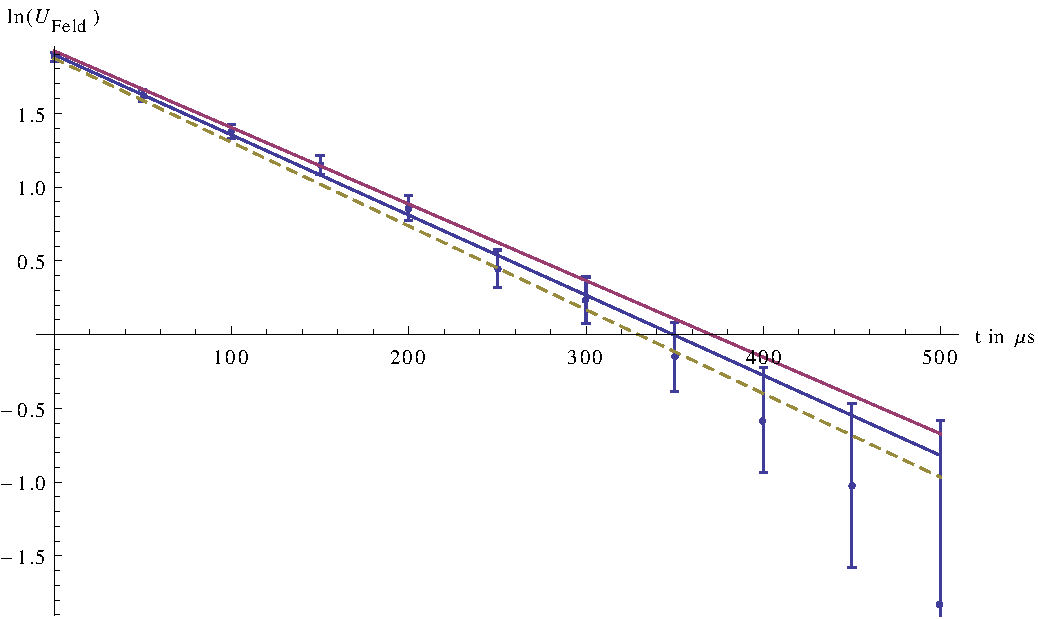
\includegraphics[width=11cm]{graph1}

Erster Doppelspalt: Abstand \(s\) der ersten 7 Maxima vom Hauptmaximum
\end{center}

\begin{center}
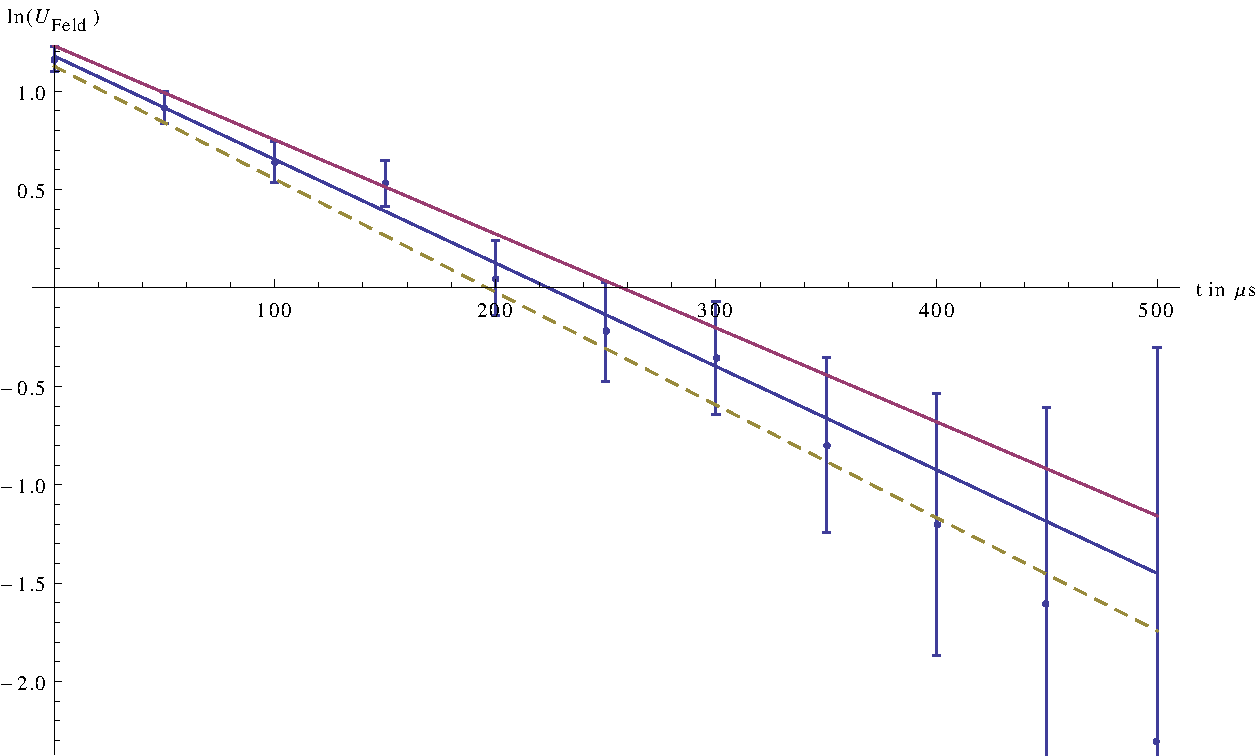
\includegraphics[width=11cm]{graph2}

Zweiter Doppelspalt: Abstand \(s\) der ersten 7 Maxima vom Hauptmaximum
\end{center}

\begin{center}
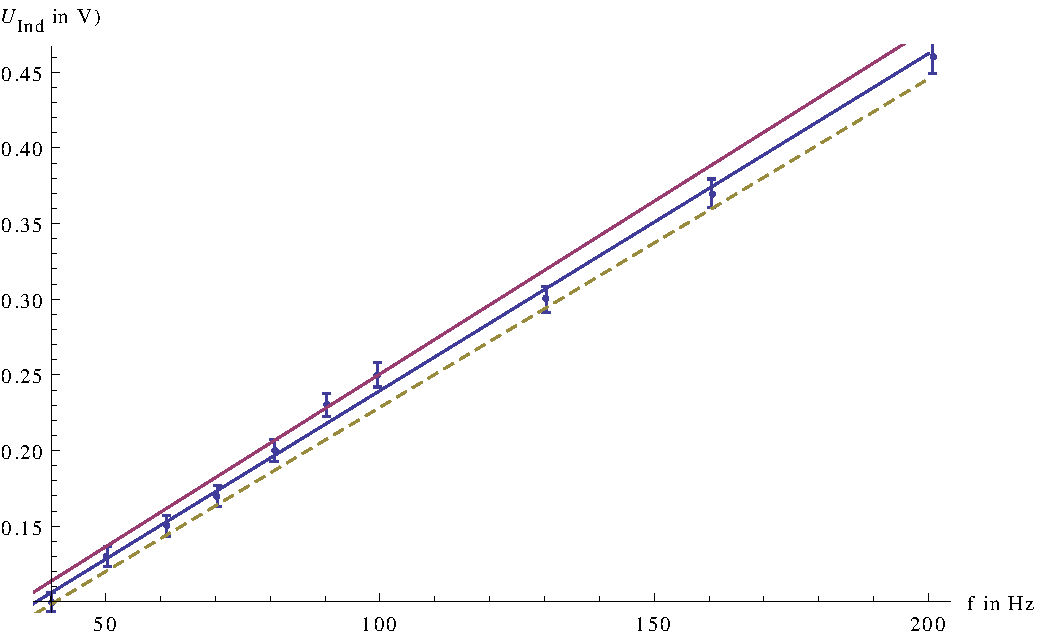
\includegraphics[width=11cm]{graph3}

Zweiter Doppelspalt: Abstand \(s\) der ersten 4 Einhüllendenmaxima vom Hauptmaximum
\end{center}

\noindent
Über die Lineare regressions Methode für Nullpunktgeraden wurden die Werte der Steigungen b für die beiden Graphen ermittelt. Für den Zweiten Doppelspalt war nur ein Einhüllendenmaxima erkennbar, daher wird der Fehler des Messwerts einfach weiter verwendet.
\begin{center}
\begin{tabular}{r c c c}
		& & Erster Doppelspalt & Zweiter Doppelspalt \\
	Feinstruktur & m	& \( (0,0120 \pm 0,0002)\,m \) 	& \( (0,0123 \pm 0,0002)\,m \) \\
	Einhüllende & m	& \( (0,0246 \pm 0,0011)\,m \) 	& \( (0,0163 \pm 0,0020)\,m \)

\end{tabular}
\end{center}

\subsection{Auswertung}
\subsubsection{Bestimmung des Spaltabstands}
Um von der Messung auf den Spaltabstande \(d\) zu kommen wird die Gleichung \eqref{alpha} mit der Näherung \eqref{sin=tan} herangezogen. Demnach gilt

\begin{equation}
\sin \alpha = \frac{s}{l}
\notag
\end{equation}

Da die Maxima der Intensität gemessen wurden kann nun mit \eqref{4} eine Funktionsgleichung aufgestellt werden. Da nur betragsmäßig die Entfernung zum Hauptmaximum durch halbieren der Abstände der Nebenmaxima voneinander errechnet wurde, wird nur der positive Term verwendet.

\begin{align}
s(n) =  \frac{\lambda l}{d} \cdot n
\notag
\end{align}

Die Steigung kann somit identifiziert werden als

\begin{align}
m =  \frac{\lambda l}{d}
\notag
\end{align}

Daraus folgt für den Parameter

\begin{align}
d =  \frac{\lambda l}{m}
\notag
\end{align}

Mit dem Fehler

\begin{align}
\Delta d &= \sqrt{
\left( \frac{\partial d}{\partial \lambda} \right)^2 +
\left( \frac{\partial d}{\partial l} \right)^2 +
\left( \frac{\partial d}{\partial m} \right)^2
} \notag \\
&=  d \cdot \sqrt{
\left( \frac{\Delta \lambda}{\lambda} \right)^2 +
\left( \frac{\Delta l}{l} \right)^2 +
\left( \frac{\Delta m}{m} \right)^2
}
\notag
\end{align}

Einsetzen der gemmessen bzw. gegebenen Daten liefert

\begin{center}
\begin{tabular}{c|c c c }
	&					& Erster Doppelspalt & Zweiter Doppelspalt \\ \hline
	Zwischenwert & \(d\)		& \( 0,2568\, mm\)	& \( 0,2505\, mm \) \\  
	Zwischenwert & \(\Delta d\)	& \( 0,0049\, mm\)	& \( 0,0047\, mm \)\\

\end{tabular}
\end{center}

\subsubsection{Bestimmung der Spaltbreite}

Die Spaltbreite wird aus dem Abstand der Einhüllendenmaxima bestimmt. Für beide Doppelspalte ist die Einhüllende Funktion jedoch nur erahnbar. Da beim zweiten Doppelspalt sogar nur ein einziges Maximum erkannbar ist, sind die Werte nur grobe Vermutungen und können nicht zur Bestätigung oder Wiederlegen der Theorie dienen.
Analog zum Spaltastand gilt nach \eqref{2} schlussendlich

\begin{align}
b &=  \frac{\lambda l}{m}
\notag
\end{align}

Mit dem Fehler

\begin{align}
\Delta b &= b \cdot \sqrt{
\left( \frac{\Delta \lambda}{\lambda} \right)^2 +
\left( \frac{\Delta l}{l} \right)^2 +
\left( \frac{\Delta m}{m} \right)^2
}
\notag
\end{align}

Einsetzen der gemmessen bzw. gegebenen Daten liefert
 
\begin{center}
\begin{tabular}{c c c c}
	&	& Erster Doppelspalt & Zweiter Doppelspalt \\
	Zwischenwert & \(b\)	& \( 0,1253\, mm\)	& \( 0,189\, mm \) \\  
	Zwischenwert & \(\Delta b\)	& \( 0,0057\, mm\)	& \( 0,023\, mm \)
\end{tabular}
\end{center}

\subsection{Fazit}

Zusammengefasst bedeutet das

\begin{center}
\begin{tabular}{c|c c c}
										&	Messgröße	& Gemessen & Gegeben \\ \hline
\multirow{2}{*}{Erster Doppelspalt}		& Spaltabstand \(d\)	& \( (0,259 \pm 0,005)\, mm \) & \(0,25\,mm\) \\
										& Spaltbreite \(b\)	& \( (0,125 \pm 0,006)\, mm \) & \(0,1\,mm\) \\	\hline
\multirow{2}{*}{Zweiter Doppelspalt}	& Spaltabstand \(d\)	& \( (0,250 \pm 0,005)\, mm \) & \(0,25\,mm\) \\
										& Spaltbreite \(b\)	& \( (0,19 \pm 0,03)\, mm \) & \(0,2\,mm\)
\end{tabular}
\end{center}

Die Messwerte des Ersten Doppelspalts weichen von den angegebenen Daten ab, dabei ist der Wert des Spaltabstrands noch verträglich, die Spaltbreite jedoch signifikant unterschiedlich. Eine mögliche Ursache dafür ist, dass die Einhüllende nicht richtig erkannt wurde und dadurch falsche Messwete verwendet wurden. Beim zweiten Doppelspalt sind die Messwerte und die Angaben gleich. Auch wenn wir nur ein Einhüllendenmaxima erkennen konnten war dies jedoch zumindest sehr gut Messbar.

%\includegraphics{/mnt/svr/svr/dominik/uni/sarah/Graph_dest}
%\putpic{-10}{20}{230}{/mnt/svr/svr/dominik/uni/sarah/Graph_dest}


\subsection{Aufgabe 3}

Für diese Aufgabe modifizieren wir den Versuchsaufbau (Skizze im Anhang), sodass nicht mehr der der X-Y-Schreiber die Messung durchführt, sondern auf einem Papierstreifen an der Wand die Interferenzstreifen aufgetragen werten. Zur Auswertung wurden die Abstände der einzelnen Maxima zur 0. Ordnung gemessen. Die Distanz zwischen Laser und der Wand betrugen dabei ohne Ablenkung e=(572,0 \(\pm\) 2,5)cm. Der Abstand vom Wandaufpunkt bis zum Maximum der 0. Ordnung betrug bei uns d=(41,7 \(\pm \) 0,5)cm, womit wir alles haben um den Einfallswinkel \(\varepsilon \) zu berechnen.

\begin{equation}
\varepsilon = \frac {1}{2} arctan \left( \frac {d}{e} \right ) 
\end{equation} \\

Wir erhielten einen Wert von \(\varepsilon = 2,08 ^\circ \). Der Fehler von \(\varepsilon \) berechnet sich wie üblich aus der Gauß'schen Fehlerfortpflanzung

\begin{equation}
\Delta \varepsilon = \frac {1}{2} \sqrt { \frac {e^2 \Delta d^2 +d^2 \Delta e^2}{ (d^2 +e^2) ^2}}
\end{equation} \\

und wir erhielten \(\Delta \varepsilon =0,25 ^\circ \). Anschließend berechnen wir den Ablenkwinkel \(\alpha \) über die Relation

\begin{equation}
\alpha = arctan \left ( \frac {d+a}{e} \right ) -2 \varepsilon
\end{equation} \\

Auch hier errechnet sich der Fehler über die Gauß'sche Fehlerfortpflanzung

\begin{equation}
\Delta \alpha = \sqrt { \frac { \Delta a^2 + \Delta d^2 }{ \left (1+ \frac{ (a+d)^2}{e^2} \right )^2 \cdot e^2}+ \frac { (a+d)^2}{ \left (1+ \frac{(a+d)^2}{e^2} \right )^2 \cdot e^4} +4 \Delta \varepsilon ^2}
\end{equation} \\

Die aufgezeichneten Werte werden in der folgenden Tabelle aufgeführt und verarbeitet, wobei a und b die Abstände der Hauptmaxima von der 1. Ordnung bei einem Abstand von 1[mm] bzw 0,5[mm] sind.

\begin{center}
\begin{tabular}{|c|c|c|c|c|c|c|}

\hline 
Ordnung & a[cm] & \(\Delta \)a[cm] & \(\alpha [^ \circ ] \) & \(\Delta \alpha [^ \circ ] \) & cos(\(\alpha \)+\(\varepsilon \)) & \(\Delta \)cos (\(\alpha \)+\(\varepsilon \)) \\
\hline 
\(1\) &	\(7.4\) &	\(0.5\) &	\(0.74619\) &	\(0.00174\) &	\(0.99878\) &	\(0.00180\)  \\  
\(2\) &	\(13.2\) &	\(0.4\) &	\(1.32239\) &	\(0.00207\) &	\(0.99823\) &	\(0.00212\)  \\  
\(3\) &	\(18.0\) &	\(0.3\) &	\(1.79842\) &	\(0.00202\) &	\(0.99771\) &	\(0.00207\)  \\ 
\(4\) &	\(22.4\) &	\(0.3\) &	\(2.23405\) &	\(0.00198\) &	\(0.99717\) &	\(0.00203\)  \\  
\(5\) &	\(26.4\) &	\(0.3\) &	\(2.62944\) &	\(0.00195\) &	\(0.99662\) &	\(0.00201\)  \\  
\(6\) &	\(30.1\) &	\(0.3\) &	\(2.99446\) &	\(0.00194\) &	\(0.99608\) &	\(0.00198\)  \\  
\hline
\end{tabular}

Tabelle 3.1: Messergebnisse der Beugung am Gitter der 1[mm] Skala 
\end{center}

\vspace{0,5cm}

\begin{center}
\begin{tabular}{|c|c|c|c|c|c|c|}

\hline 
Ordnung & a[cm] & \(\Delta \)a[cm] & \(\alpha [^ \circ ] \) & \(\Delta \alpha [^ \circ ] \) & cos(\(\alpha \)+\(\varepsilon \)) & \(\Delta \)cos (\(\alpha \)+\(\varepsilon \)) \\
\hline 
\(1\) &	\(12.8\) &	\(0.5\) &	\(1.24369\) &	\(0.00174\) &	\(0.9983\) &	\(0.0018\)  \\
\(2\) &	\(22.2\) &	\(0.3\) &	\(2.17469\) &	\(0.00174\) &	\(0.9972\) &	\(0.0018\)  \\
\(3\) &	\(30.1\) &	\(0.3\) &	\(2.95515\) &	\(0.00174\) &	\(0.9961\) &	\(0.0018\)  \\
\(4\) &	\(36.9\) &	\(0.4\) &	\(3.62483\) &	\(0.00174\) &	\(0.9950\) &	\(0.0018\)  \\
\(5\) &	\(43.1\) &	\(0.5\) &	\(4.23357\) &	\(0.00174\) &	\(0.9939\) &	\(0.0018\)  \\
\(6\) &	\(48.3\) &	\(0.4\) &	\(4.74365\) &	\(0.00174\) &	\(0.9929\) &	\(0.0018\)  \\
\hline

\end{tabular}
Tabelle 3.2: Messergebnisse der Beugung am Gitter der 0.5 [mm] Skala
\end{center}

Nun wollen wir die Teilungsabstände der Skala berechnen und stellen hierfür Gl.\(\eqref{5}\) einfach nach d um und erhalten

\begin{equation}
\label{6}
d = \frac {z \lambda}{ ( cos \varepsilon - cos( \varepsilon + a))}
\end{equation}

\newpage

Nun tragen wir die, um das Ergebnis graphisch zu bestimmen, den \(\ cos(\alpha + \varepsilon ) \) über die Ordnungszahl der Hauptmaxima ab, wobei uns die Steigung 


\begin{equation}
\label{20}
m= - \frac{\lambda }{d}
\end{equation}

\begin{figure}[htbp]
\centering
\includegraphics[scale=0.5]{a3graph1}
\begin{center}
\caption{Winkel über Ordnungszahlzur Bestimmung von\(\ m_{1} \)}
\end{center}

\centering
\includegraphics[scale=0.5]{a3graph2}
\begin{center}
\caption{Winkel über Ordnungszahlzur Bestimmung von\(\ m_{2} \)}
\end{center}
\end{figure}

\newpage

Für die Steigung erhalten wir nun

\begin{center}
\(\ m_{a}=(-0,00054 \pm 0,0005) \)
\end{center}

\begin{center}
\(\ m_{b}=(-0,00109 \pm 0,0042) \)
\end{center}

 Gl.\(\eqref{20}\) nun noch nach d umstellen liefert uns die Teilungsabstände

\begin{center}
\(\ d_{a}=(1,007 \pm 0,006)mm \)
\end{center}

\begin{center}
\(\ d_{b}=(0,498 \pm 0,003)mm \)
\end{center}

Der Fehler berechnet sich wie zuvor mit der Gauß'schen Fehlerfortpflanzung über die Formel

\begin{equation}
\Delta d= \sqrt{\left ( \frac{ \Delta \lambda}{\lambda} \right )^2+\left (\frac {\Delta m}{m} \right )^2} \cdot d
\end{equation}

\subsection{Fazit}

Die errechneten Werte für die Teilungsabständen liegen im einfachen Fehlerintervall und sind somit ziemlich genau. Der Versuch war im Allgemeinen, bis vielleicht auf die Schwierigkeiten des Messens der Distanz zwischen dem Laser und der Wand, ziemlich erfolgreich. In den Abbildungen 1 und 2 der Aufzeichnungen (siehe Anhang) war es recht schwer eine passende Einhüllende einzuzeichnen, weswegen wir in der Aufgabe 1 verschiedene Abweichungen bekamen.

\newpage
\section{Anhang}

\begin{figure}[htbp]
\centering
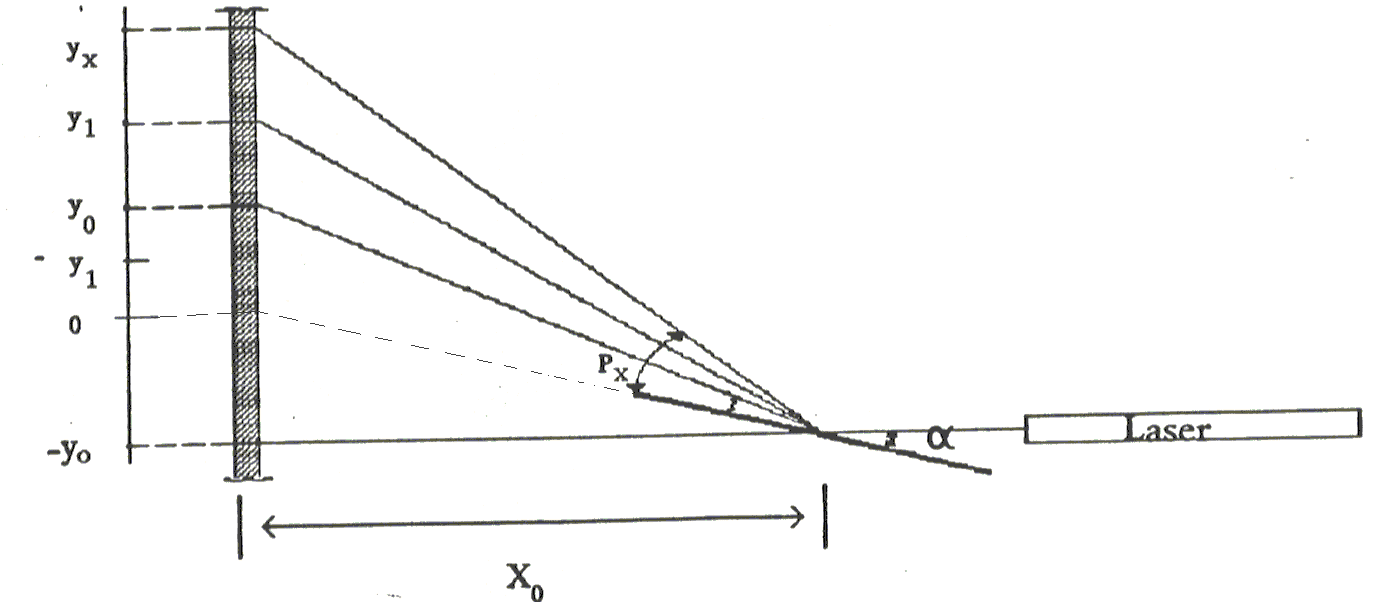
\includegraphics[scale=0.3]{BEU6.png}
\begin{center}
\caption{Versuchsaufbau Aufgabe 3}
\end{center}
\end{figure}
\end{document}